\documentclass{standalone}
\usepackage{tikz}
\usetikzlibrary{patterns, positioning}


\begin{document}
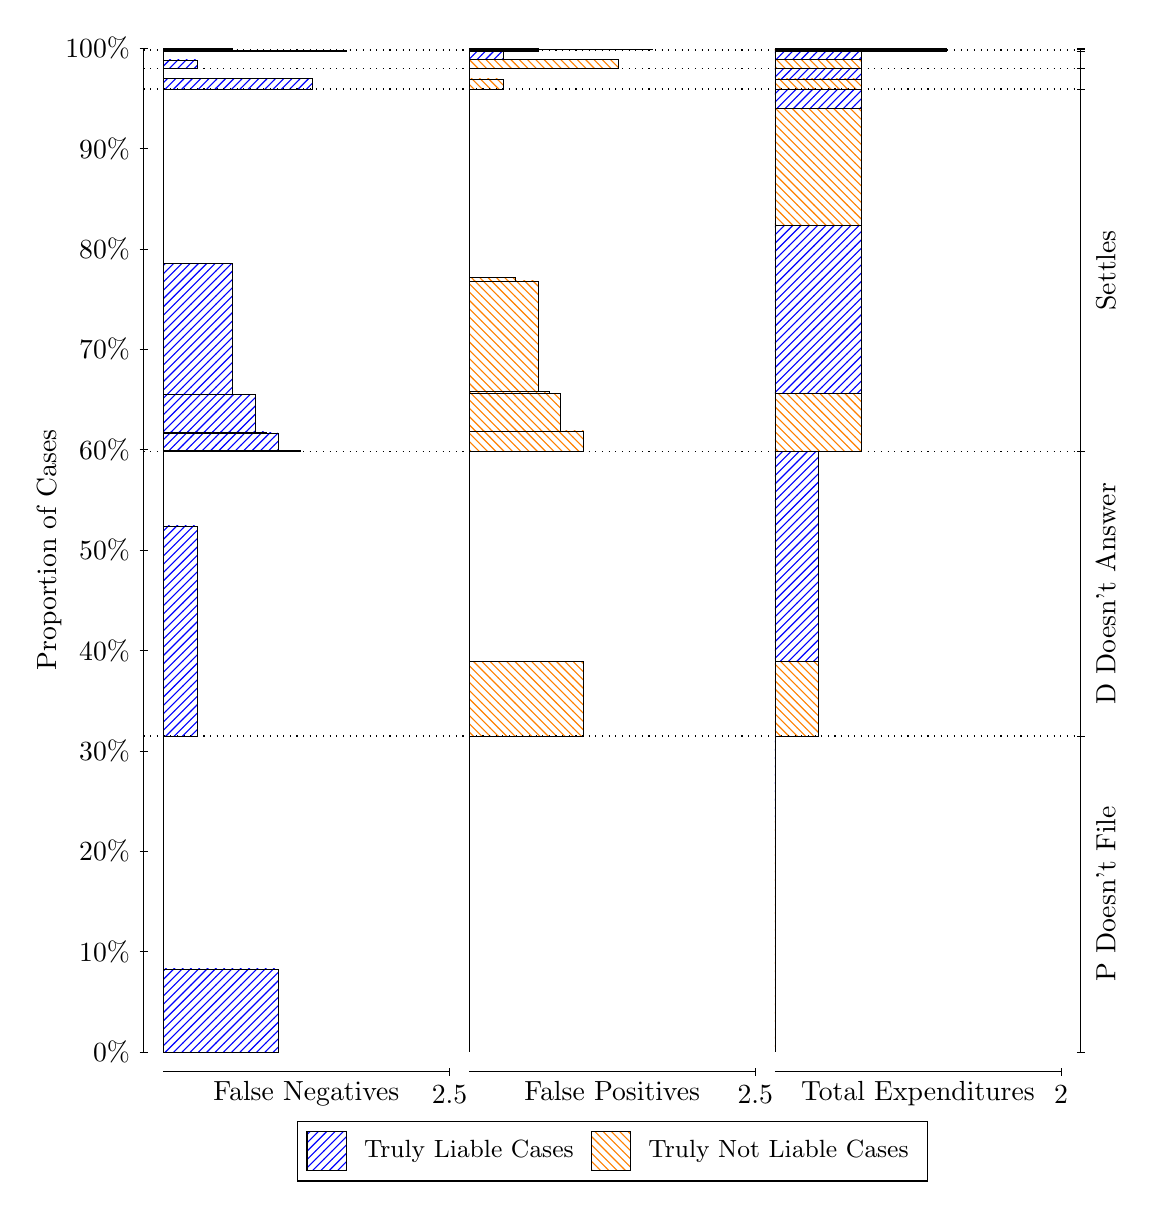
\begin{tikzpicture}
\draw[black, very thin] (1.5,1.75) -- (1.5,14.5);
\node[rotate=90, text=black, anchor=center] at (0.3, 8.125) {Proportion of Cases};
\draw[black, very thin] (1.45,1.75) -- (1.55,1.75);
\node[text=black, anchor=east] at (1.45, 1.75) {0\%};
\draw[black, very thin] (1.45,3.025) -- (1.55,3.025);
\node[text=black, anchor=east] at (1.45, 3.025) {10\%};
\draw[black, very thin] (1.45,4.3) -- (1.55,4.3);
\node[text=black, anchor=east] at (1.45, 4.3) {20\%};
\draw[black, very thin] (1.45,5.575) -- (1.55,5.575);
\node[text=black, anchor=east] at (1.45, 5.575) {30\%};
\draw[black, very thin] (1.45,6.85) -- (1.55,6.85);
\node[text=black, anchor=east] at (1.45, 6.85) {40\%};
\draw[black, very thin] (1.45,8.125) -- (1.55,8.125);
\node[text=black, anchor=east] at (1.45, 8.125) {50\%};
\draw[black, very thin] (1.45,9.4) -- (1.55,9.4);
\node[text=black, anchor=east] at (1.45, 9.4) {60\%};
\draw[black, very thin] (1.45,10.675) -- (1.55,10.675);
\node[text=black, anchor=east] at (1.45, 10.675) {70\%};
\draw[black, very thin] (1.45,11.95) -- (1.55,11.95);
\node[text=black, anchor=east] at (1.45, 11.95) {80\%};
\draw[black, very thin] (1.45,13.225) -- (1.55,13.225);
\node[text=black, anchor=east] at (1.45, 13.225) {90\%};
\draw[black, very thin] (1.45,14.5) -- (1.55,14.5);
\node[text=black, anchor=east] at (1.45, 14.5) {100\%};

\draw[black, very thin] (13.4,1.75) -- (13.4,14.5);
\draw[black, very thin] (13.35,1.75) -- (13.45,1.75);
\node[anchor=west] at (13.35, 1.75) {};
\draw[black, very thin] (13.35,5.7628) -- (13.45,5.7628);
\node[anchor=west] at (13.35, 5.7628) {};
\draw[black, very thin] (13.35,9.3734) -- (13.45,9.3734);
\node[anchor=west] at (13.35, 9.3734) {};
\draw[black, very thin] (13.35,13.98) -- (13.45,13.98);
\node[anchor=west] at (13.35, 13.98) {};
\draw[black, very thin] (13.35,14.244) -- (13.45,14.244);
\node[anchor=west] at (13.35, 14.244) {};
\draw[black, very thin] (13.35,14.463) -- (13.45,14.463);
\node[anchor=west] at (13.35, 14.463) {};
\draw[black, very thin] (13.35,14.481) -- (13.45,14.481);
\node[anchor=west] at (13.35, 14.481) {};
\draw[black, very thin] (13.35,14.5) -- (13.45,14.5);
\node[anchor=west] at (13.35, 14.5) {};

\draw[black, very thin, pattern color=blue, pattern=north east lines] (1.75,1.75) rectangle (3.2033,2.8046);
\draw[black, very thin, pattern color=orange, pattern=north west lines] (1.75,2.8046) rectangle (1.75,5.7628);
\draw[black, very thin, pattern color=blue, pattern=north east lines] (1.75,5.7628) rectangle (2.186,8.4307);
\draw[black, very thin, pattern color=orange, pattern=north west lines] (1.75,8.4307) rectangle (1.75,9.3734);
\draw[black, very thin, pattern color=blue, pattern=north east lines] (1.75,9.3734) rectangle (3.494,9.3862);
\draw[black, very thin, pattern color=blue, pattern=north east lines] (1.75,9.3862) rectangle (3.2033,9.6136);
\draw[black, very thin, pattern color=blue, pattern=north east lines] (1.75,9.6136) rectangle (3.058,9.6253);
\draw[black, very thin, pattern color=blue, pattern=north east lines] (1.75,9.6253) rectangle (2.9127,10.1);
\draw[black, very thin, pattern color=blue, pattern=north east lines] (1.75,10.1) rectangle (2.622,11.764);
\draw[black, very thin, pattern color=orange, pattern=north west lines] (1.75,11.764) rectangle (1.75,13.98);
\draw[black, very thin, pattern color=blue, pattern=north east lines] (1.75,13.98) rectangle (3.6393,14.117);
\draw[black, very thin, pattern color=orange, pattern=north west lines] (1.75,14.117) rectangle (1.75,14.244);
\draw[black, very thin, pattern color=blue, pattern=north east lines] (1.75,14.244) rectangle (2.186,14.349);
\draw[black, very thin, pattern color=orange, pattern=north west lines] (1.75,14.349) rectangle (1.75,14.463);
\draw[black, very thin, pattern color=blue, pattern=north east lines] (1.75,14.463) rectangle (4.0753,14.469);
\draw[black, very thin, pattern color=orange, pattern=north west lines] (1.75,14.469) rectangle (1.75,14.481);
\draw[black, very thin, pattern color=blue, pattern=north east lines] (1.75,14.481) rectangle (2.622,14.494);
\draw[black, very thin, pattern color=orange, pattern=north west lines] (1.75,14.494) rectangle (1.75,14.5);
\draw[black, very thin, pattern color=orange, pattern=north west lines] (5.6333,1.75) rectangle (5.6333,4.7083);
\draw[black, very thin, pattern color=blue, pattern=north east lines] (5.6333,4.7083) rectangle (5.6333,5.7628);
\draw[black, very thin, pattern color=orange, pattern=north west lines] (5.6333,5.7628) rectangle (7.0867,6.7055);
\draw[black, very thin, pattern color=blue, pattern=north east lines] (5.6333,6.7055) rectangle (5.6333,9.3734);
\draw[black, very thin, pattern color=orange, pattern=north west lines] (5.6333,9.3734) rectangle (7.0867,9.6364);
\draw[black, very thin, pattern color=orange, pattern=north west lines] (5.6333,9.6364) rectangle (6.796,10.113);
\draw[black, very thin, pattern color=orange, pattern=north west lines] (5.6333,10.113) rectangle (6.6507,10.136);
\draw[black, very thin, pattern color=orange, pattern=north west lines] (5.6333,10.136) rectangle (6.5053,11.543);
\draw[black, very thin, pattern color=orange, pattern=north west lines] (5.6333,11.543) rectangle (6.2147,11.589);
\draw[black, very thin, pattern color=blue, pattern=north east lines] (5.6333,11.589) rectangle (5.6333,13.98);
\draw[black, very thin, pattern color=orange, pattern=north west lines] (5.6333,13.98) rectangle (6.0693,14.107);
\draw[black, very thin, pattern color=blue, pattern=north east lines] (5.6333,14.107) rectangle (5.6333,14.244);
\draw[black, very thin, pattern color=orange, pattern=north west lines] (5.6333,14.244) rectangle (7.5227,14.358);
\draw[black, very thin, pattern color=blue, pattern=north east lines] (5.6333,14.358) rectangle (6.0693,14.463);
\draw[black, very thin, pattern color=orange, pattern=north west lines] (5.6333,14.463) rectangle (6.5053,14.475);
\draw[black, very thin, pattern color=blue, pattern=north east lines] (5.6333,14.475) rectangle (5.6333,14.481);
\draw[black, very thin, pattern color=orange, pattern=north west lines] (5.6333,14.481) rectangle (7.9587,14.486);
\draw[black, very thin, pattern color=blue, pattern=north east lines] (5.6333,14.486) rectangle (6.5053,14.5);
\draw[black, very thin, pattern color=orange, pattern=north west lines] (9.5167,1.75) rectangle (9.5167,4.7083);
\draw[black, very thin, pattern color=blue, pattern=north east lines] (9.5167,4.7083) rectangle (9.5167,5.7628);
\draw[black, very thin, pattern color=orange, pattern=north west lines] (9.5167,5.7628) rectangle (10.062,6.7055);
\draw[black, very thin, pattern color=blue, pattern=north east lines] (9.5167,6.7055) rectangle (10.062,9.3734);
\draw[black, very thin, pattern color=orange, pattern=north west lines] (9.5167,9.3734) rectangle (10.607,10.113);
\draw[black, very thin, pattern color=blue, pattern=north east lines] (9.5167,10.113) rectangle (10.607,12.252);
\draw[black, very thin, pattern color=orange, pattern=north west lines] (9.5167,12.252) rectangle (10.607,13.729);
\draw[black, very thin, pattern color=blue, pattern=north east lines] (9.5167,13.729) rectangle (10.607,13.98);
\draw[black, very thin, pattern color=orange, pattern=north west lines] (9.5167,13.98) rectangle (10.607,14.107);
\draw[black, very thin, pattern color=blue, pattern=north east lines] (9.5167,14.107) rectangle (10.607,14.244);
\draw[black, very thin, pattern color=orange, pattern=north west lines] (9.5167,14.244) rectangle (10.607,14.358);
\draw[black, very thin, pattern color=blue, pattern=north east lines] (9.5167,14.358) rectangle (10.607,14.463);
\draw[black, very thin, pattern color=orange, pattern=north west lines] (9.5167,14.463) rectangle (11.697,14.475);
\draw[black, very thin, pattern color=blue, pattern=north east lines] (9.5167,14.475) rectangle (11.697,14.481);
\draw[black, very thin, pattern color=orange, pattern=north west lines] (9.5167,14.481) rectangle (11.697,14.486);
\draw[black, very thin, pattern color=blue, pattern=north east lines] (9.5167,14.486) rectangle (11.697,14.5);
\draw[black, dotted] (1.5,5.7628) -- (13.4,5.7628);
\draw[black, dotted] (1.5,9.3734) -- (13.4,9.3734);
\draw[black, dotted] (1.5,13.98) -- (13.4,13.98);
\draw[black, dotted] (1.5,14.244) -- (13.4,14.244);
\draw[black, dotted] (1.5,14.463) -- (13.4,14.463);
\draw[black, dotted] (1.5,14.481) -- (13.4,14.481);
\draw[black, very thin] (1.75,1.5) -- (5.3833,1.5);
\node[text=black, anchor=north] at (3.5667, 1.5) {False Negatives};
\draw[black, very thin] (5.3833,1.45) -- (5.3833,1.55);
\node[text=black, anchor=north] at (5.3833, 1.45) {2.5};

\draw[black, very thin] (5.6333,1.5) -- (9.2667,1.5);
\node[text=black, anchor=north] at (7.45, 1.5) {False Positives};
\draw[black, very thin] (9.2667,1.45) -- (9.2667,1.55);
\node[text=black, anchor=north] at (9.2667, 1.45) {2.5};

\draw[black, very thin] (9.5167,1.5) -- (13.15,1.5);
\node[text=black, anchor=north] at (11.333, 1.5) {Total Expenditures};
\draw[black, very thin] (13.15,1.45) -- (13.15,1.55);
\node[text=black, anchor=north] at (13.15, 1.45) {2};

\node[text=black, centered, rotate=90] at (13.72, 3.7564) {P Doesn't File};
\node[text=black, centered, rotate=90] at (13.72, 7.5681) {D Doesn't Answer};
\node[text=black, centered, rotate=90] at (13.72, 11.677) {Settles};





\draw (7.449999999999999,1.5) node[draw=none] (baseCoordinate) {};
\begin{scope}[align=center]
        \matrix[scale=0.5, draw=black, below=0.5cm of baseCoordinate, nodes={draw}, column sep=0.1cm]{
            \node[rectangle, draw, minimum width=0.5cm, minimum height=0.5cm, pattern color=blue, pattern=north east lines] {}; &
            \node[draw=none, font=\small, text=black] (B) {Truly Liable Cases}; &
            \node[rectangle, draw, minimum width=0.5cm, minimum height=0.5cm, pattern color=orange, pattern=north west lines] {}; &
            \node[draw=none, font=\small, text=black] (B) {Truly Not Liable Cases}; \\
            };
\end{scope}

\end{tikzpicture}
\end{document}